\documentclass[tikz,border=2pt]{standalone}
\usepackage{amsmath,amssymb}
\usepackage{pgfplots}
\pgfplotsset{compat=1.18}
\usetikzlibrary{arrows.meta}
\begin{document}
% Franchise deductible d = 100: payment Y^L = X 1{X > d} is 0 up to d and jumps to the full loss above d
% (80 -> 0, 150 -> 150); the ordinary deductible (X - d)_+ pays 0 and 50.
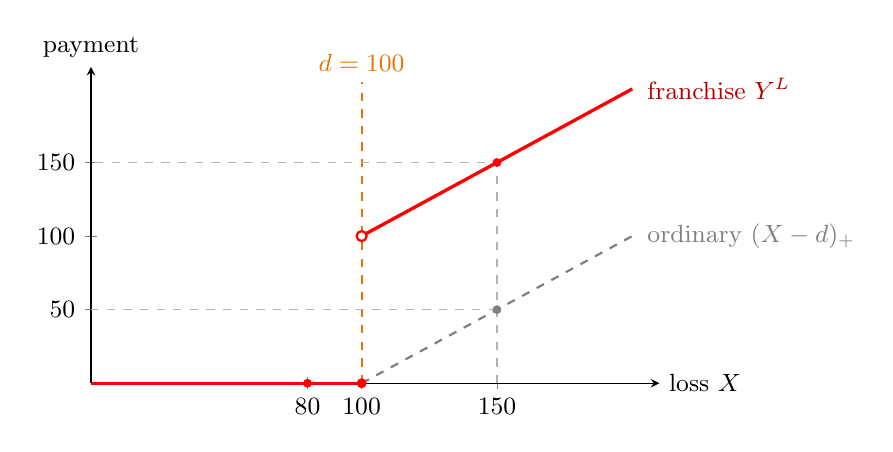
\begin{tikzpicture}[font=\small, >={Latex[length=2mm]}]
  \begin{axis}[
    axis lines=left, xmin=0, xmax=210, ymin=0, ymax=215,
    xtick={80,100,150}, ytick={50,100,150},
    xlabel={loss $X$}, ylabel={payment},
    xlabel style={at={(axis description cs:1,0)}, anchor=west},
    ylabel style={rotate=-90, at={(axis description cs:0,1)}, anchor=south},
    width=8.8cm, height=5.6cm, clip=false
    ]
    \draw[orange!90!black, thick, dashed] (axis cs:100,0) -- (axis cs:100,205);
    \node[orange!90!black, anchor=south] at (axis cs:100,205) {$d=100$};
    \addplot[gray, thick, dashed, domain=100:200, samples=2] {x-100};
    \draw[red, very thick] (axis cs:0,0) -- (axis cs:100,0);
    \draw[red, very thick] (axis cs:100,100) -- (axis cs:200,200);
    \draw[red, thick, fill=white] (axis cs:100,100) circle (1.8pt);
    \fill[red] (axis cs:100,0) circle (1.8pt);
    \draw[gray!60, thin, dashed] (axis cs:150,0) -- (axis cs:150,150) -- (axis cs:0,150);
    \draw[gray!60, thin, dashed] (axis cs:150,50) -- (axis cs:0,50);
    \fill[red] (axis cs:150,150) circle (1.6pt);
    \fill[gray] (axis cs:150,50) circle (1.6pt);
    \fill[red] (axis cs:80,0) circle (1.6pt);
    \node[red!70!black, anchor=west] at (axis cs:202,200) {franchise $Y^L$};
    \node[gray, anchor=west] at (axis cs:202,100) {ordinary $(X-d)_+$};
  \end{axis}
\end{tikzpicture}
\end{document}
